\chapter{QM/MM Non-adiabatic Dynamics of PPV\(_3\)-NO\(_2\)}

\section{Introduction}

\section{Simulation Methods}

\noindent
\begin{minipage}[c]{\textwidth}
  \centering
  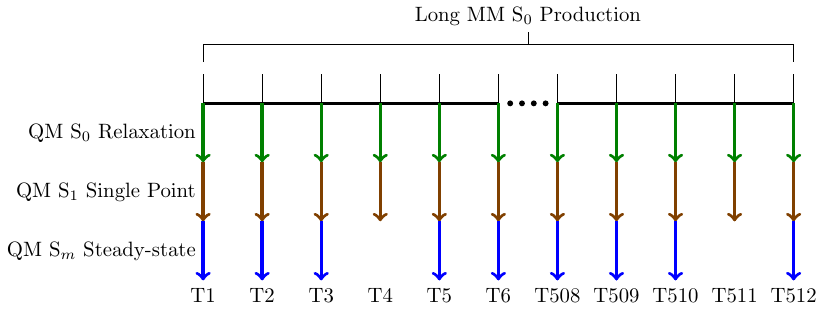
\includegraphics[width=5in]{../Paper2/scripted_diagrams/simulations-1.png}
  \captionof{figure}{Diagram of the Nonadiabatic dyanmics simulation.}
  \label{fig:nonadiabaticSimulation}
\end{minipage}\bigskip

We equilibrated the system to a temperature set to 300K. To collect a broad
enough sampling, we sampled from a 1024 ps, with a 0.5 fs timestep fully
classical trajectories using the AMBER force field. We performed a separate
trajectory for each situation combination of solute / with solvent including
whether the solvent was included in the QM calculations. We had a total of 6
separate 1024 ps classical trajectories, PPV3 in Vacuum, CH\(_3\)OH, and 5QM CH\(_3\)OH
and PPV\(_3\)-NO\(_2\) in Vacuum, CH\(_3\)OH, and 5QM CH\(_3\)OH. 1024 snapshots where taken at
1ps, 2ps .. 1024ps. We used the final frame of those tranjectories as the
initial conditions for an additional 4ps using the AM1 semiempical Hamiltonian
Born-Oppenheimer on the molecules to be included in future QM calculations to
allow the system to relax. The 4 ps timescale was determined using the
information form the previous paper. The simulations were described the Langevin
equations at a temperature set to 300 K with the Langevin friction parameter set
to 2 ps\(^{-1}\). The final frames of these QM trajectories were then used as the
initial conditions for the following pulse pump calculations.

Pump-Probe Spectroscopy is an experimental technique commonly performed in the
study of ultrafast electonic statte dynamics. In the case of conjugated polymers
in can be used to study the localized excictronic transitions that are
accessible through an excitation from the S1 state but not the ground state S0.
To simulate this behavior, we take the final snapshot of the QM ground state
calculations and perform a single point calculation at the S1 state to find the
next state with the highest oscillator strength.

The unnormalized probabilities are determined using
    \begin{equation}
      P'(\Omega_e) = f_{ge}(\Omega_e) \times \frac{1}{\sqrt{2\pi \sigma^2}} \exp \left[ - \frac{(\Omega_e - \Omega)^2}{2\sigma^2} \right]
    \end{equation}
where \(\Omega\) is the energy of the laser exciatation, \(\Omega_\alpha\) the energy difference from the ground state at excited state \(\alpha\), \(f_{ge}(\Omega_e)\) is oscillator strength, and \(\sigma\) the spectral broadening.  

The probability of initially populating an excited state \(\alpha\) is then
\begin{equation}
  P(\Omega_\alpha) = \frac{P'(\Omega_i)}{\sum_i P'(\Omega_i)}
\end{equation}

\section{Results}

\subsection{Intitial Excitations}

\noindent
\begin{minipage}[c]{\textwidth}
  \centering
  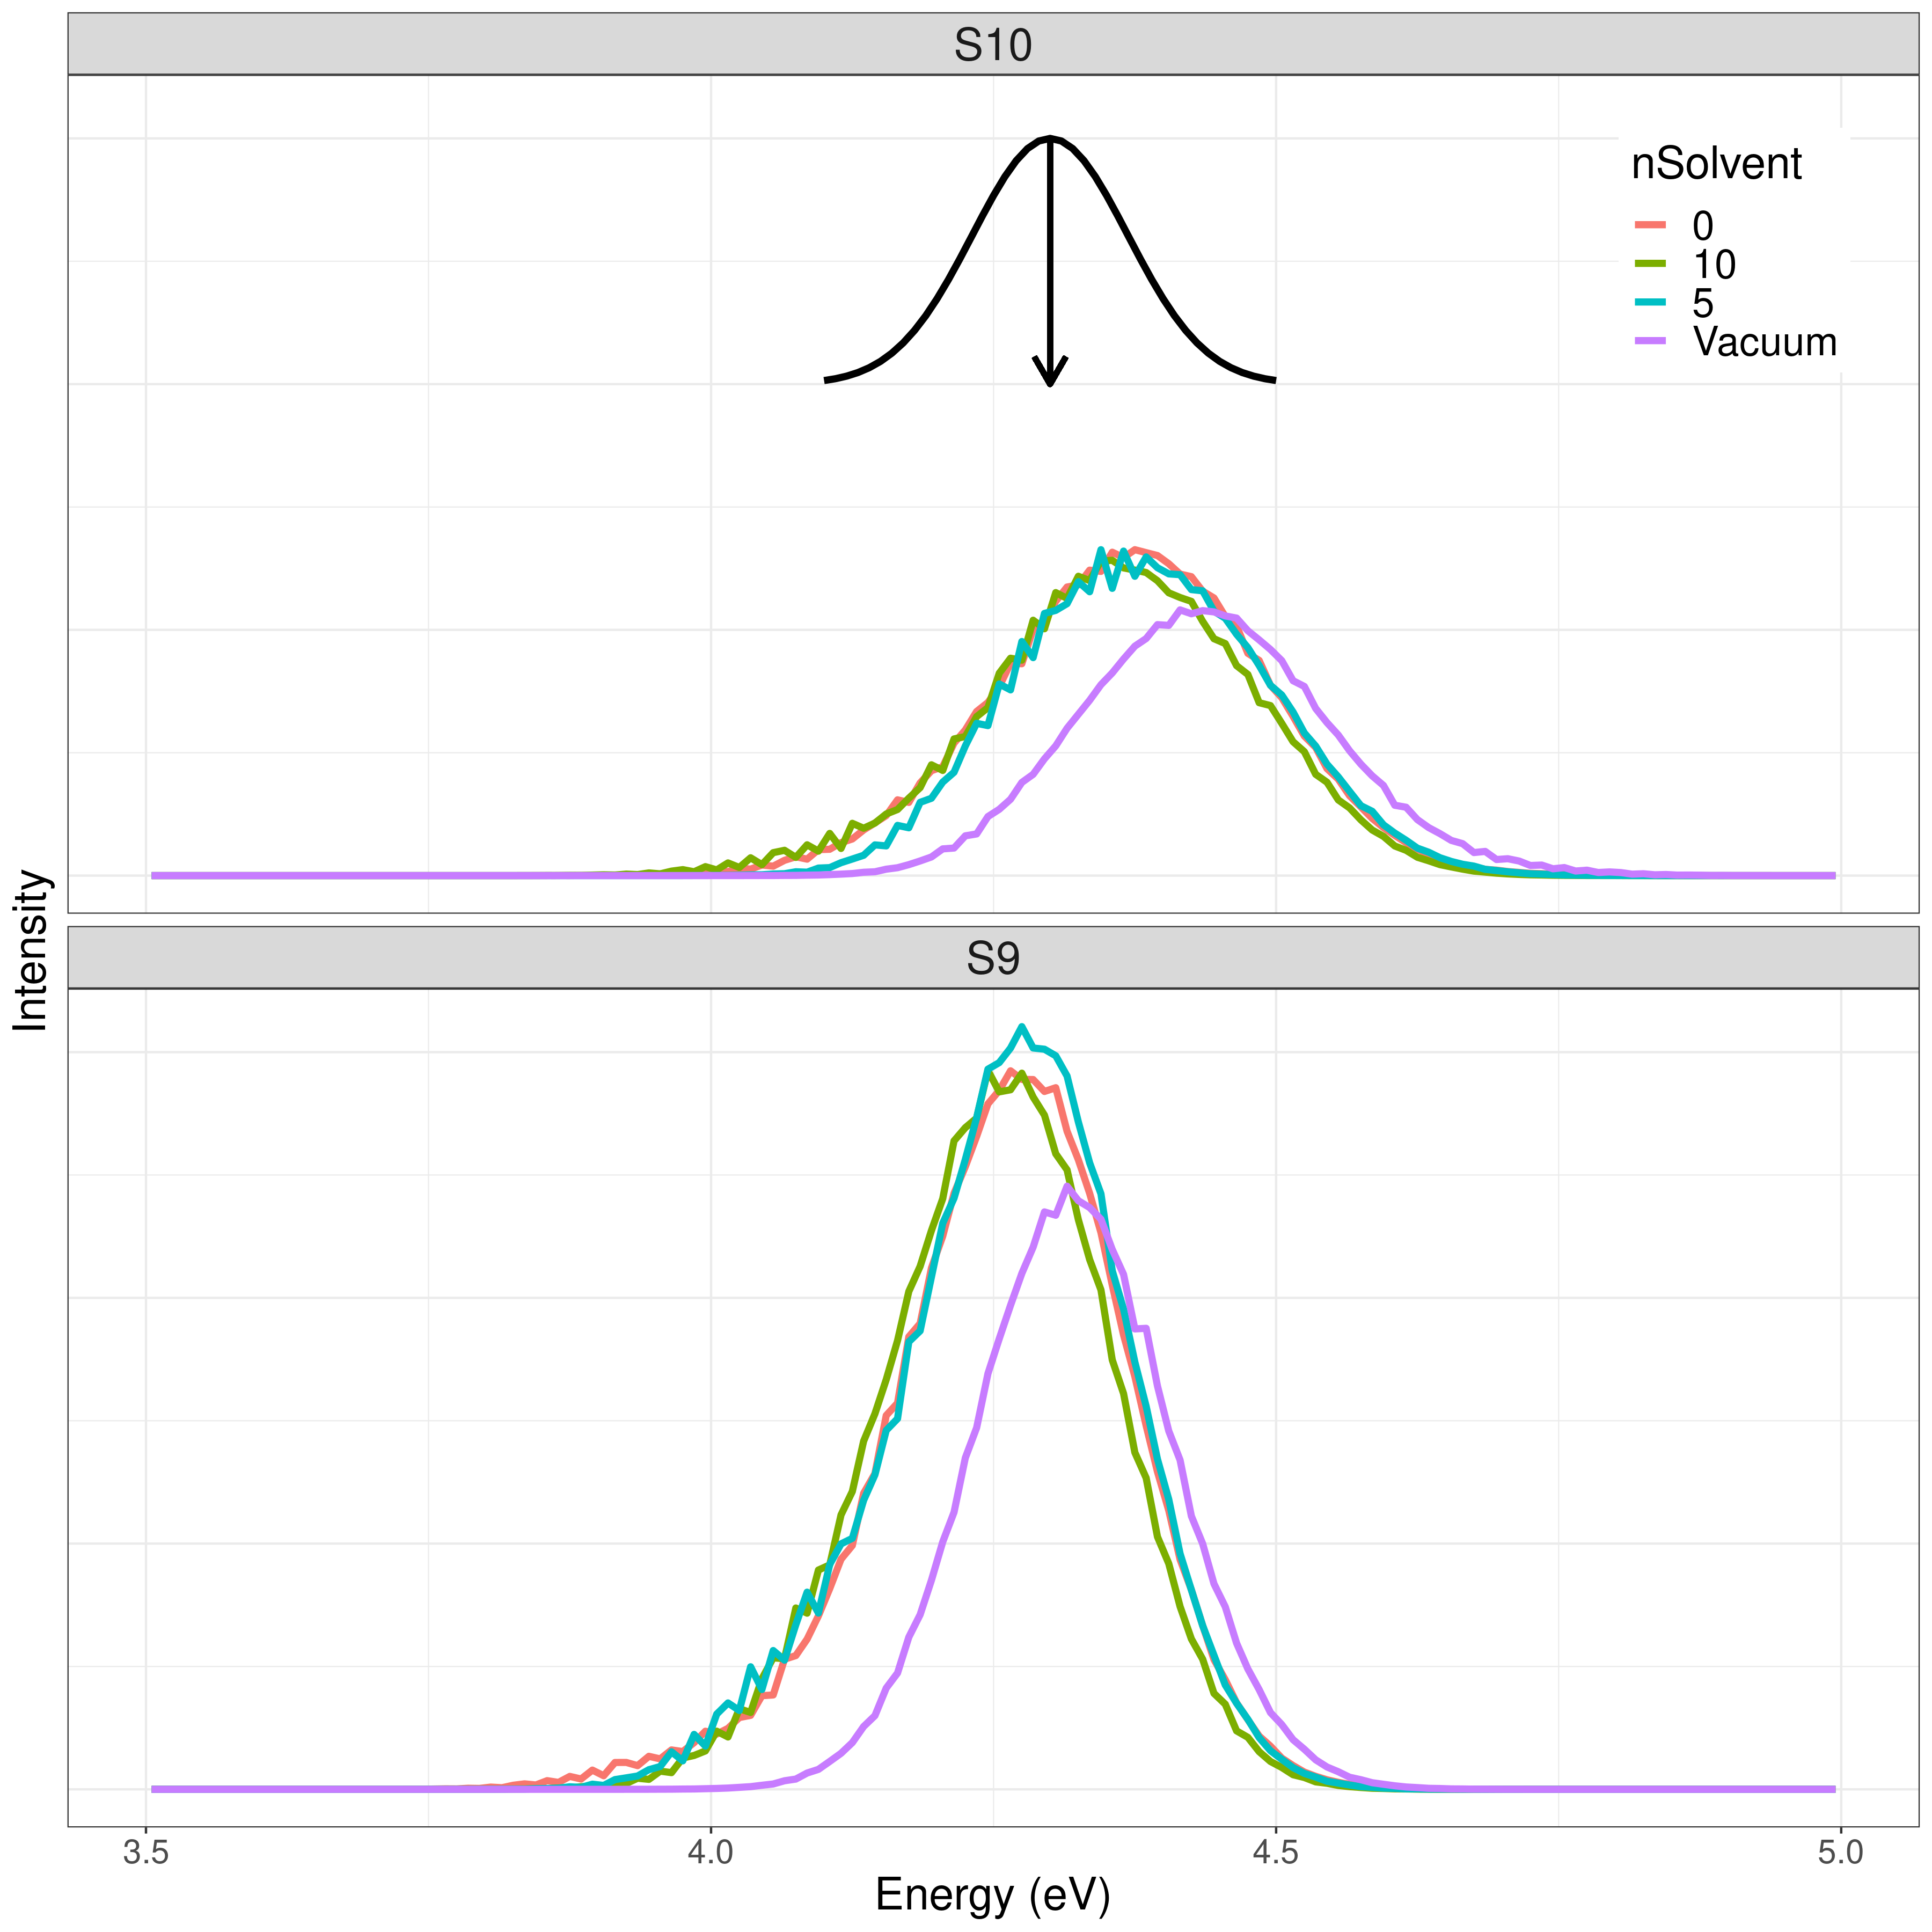
\includegraphics[width=5in]{../Paper2/Images/pulse_pump/spectra.png}
  \captionof{figure}{The calculated absorption spectrum from the first excited state S\(_1\). State energies are differences from the ground state.}
  \label{s1absorption}
\end{minipage}\bigskip

\subsection{State Population Relaxation}

\noindent
\begin{minipage}[c]{\textwidth}
  \centering
  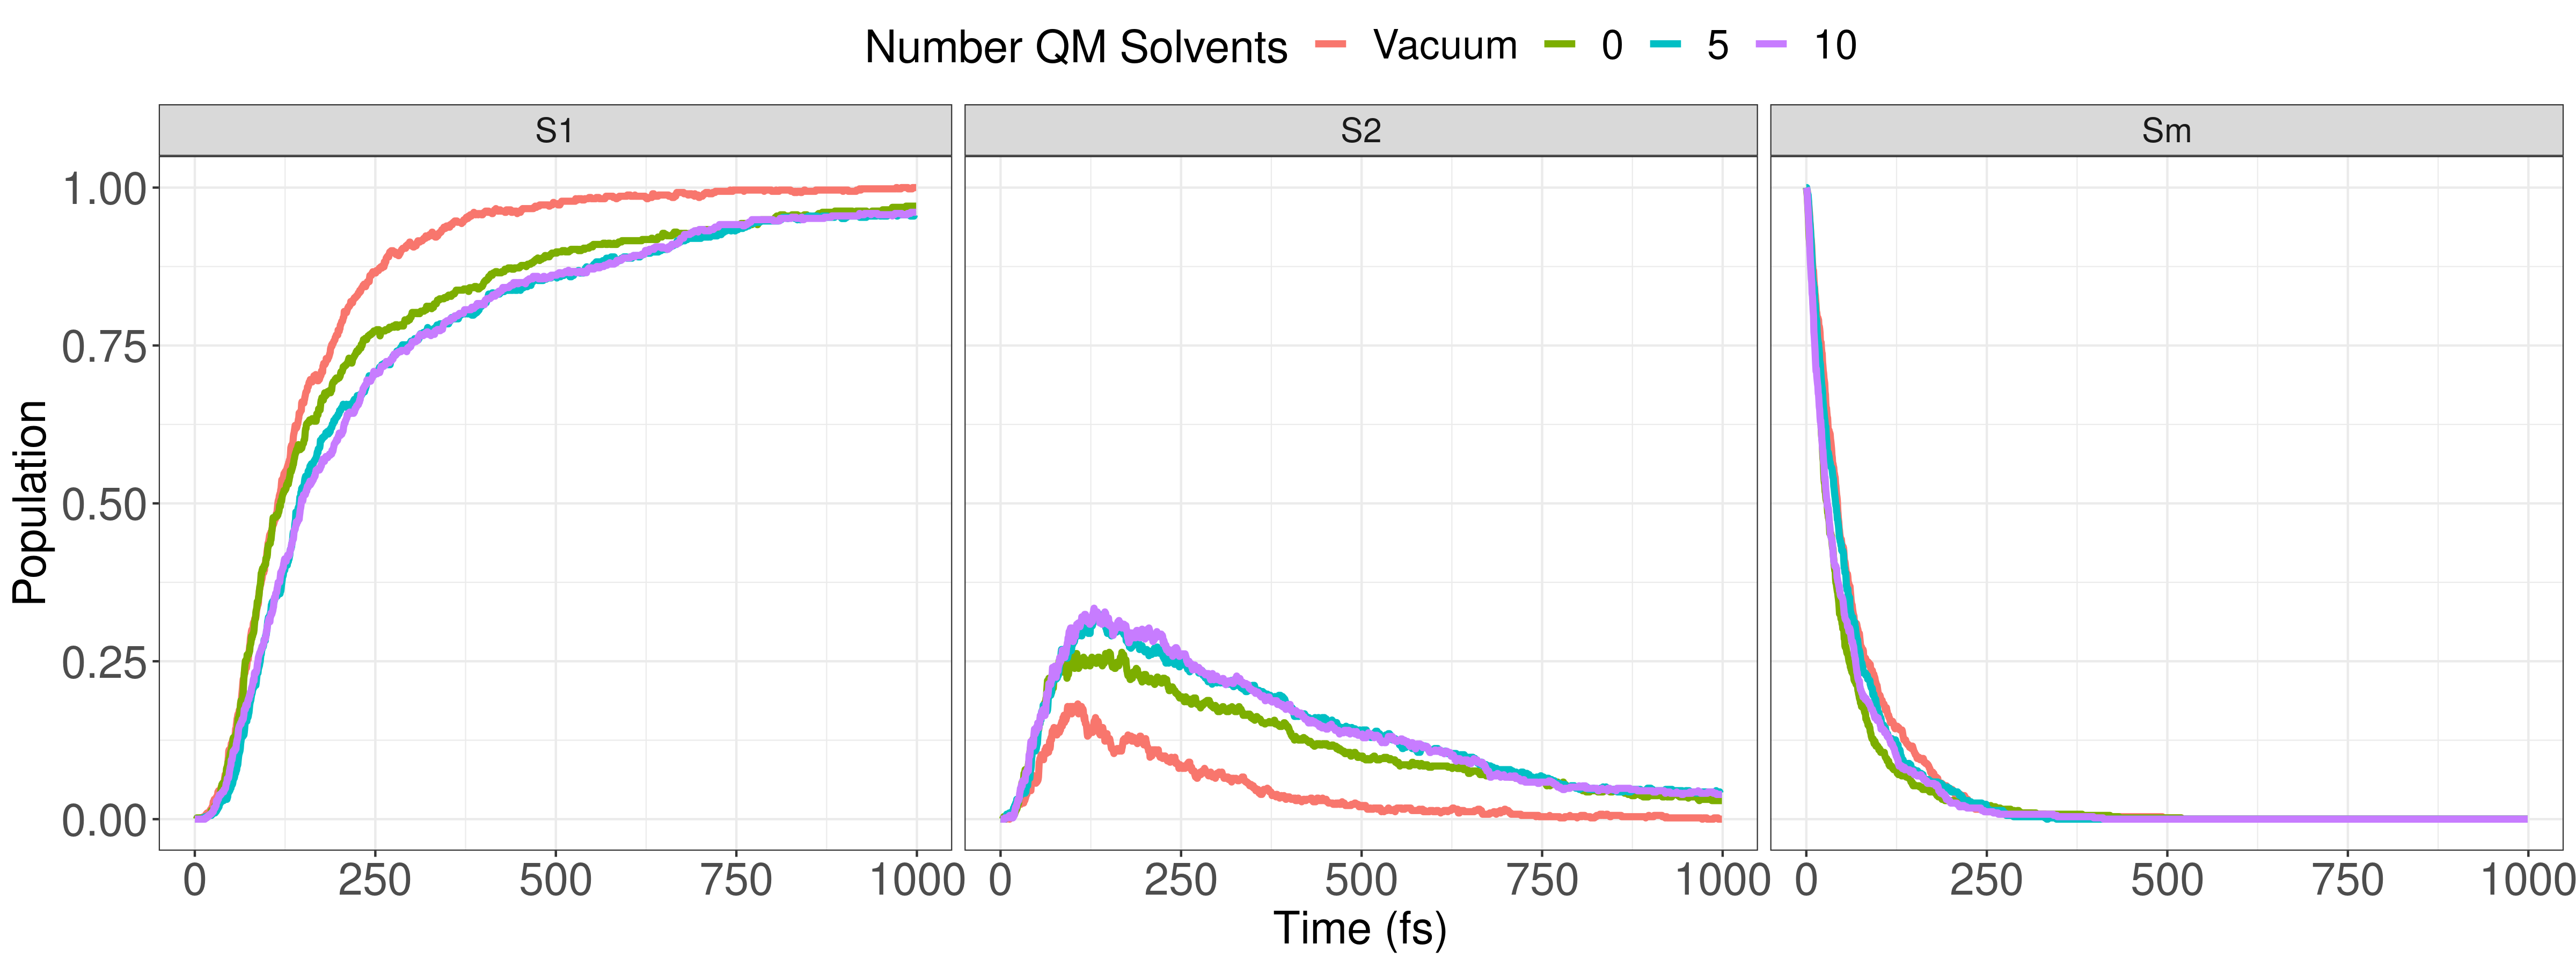
\includegraphics[width=0.9\textwidth]{../Paper2/Images/populations/solvent_comparison.png}
  \captionof{figure}[Test]{Comparison of the population decays or rises of states S\(_1\), S\(_2\), and the initial state S\(_m\) between simulations with varying number of solvents included in the QM region.}
  \label{stateDecay}
\end{minipage}\bigskip

Figure ref:fig:all-populations shows the population of each state calculated as
the number of trajectories at the state's potential energy surface over the
total number of trajectories. S\(_m\) represents the initial state calculated using
the pulse pump calculations previously done. States S\(_7\) and S\(_9\) are included as
the only other "slow" states, or states that reached a population of more than
0.05. The other states were excluded from the graph. These charts show that the
addition of the NO\(_2\) oligimors dramatically speed up the state relaxation. S\(_m\)
ranged from S\(_9\) to S\(_15\) for PPV\(_3\) and S\(_11\) to S\(_21\) for PPV\(_{3}\)-NO\(_{2}\). Figure
ref:fig:s1-populations, shows the rise of the S\(_{1}\) populations over the first
500 fs after excitation. We model these rises by fitting the curves to the
function
\begin{equation}
f(t) = \frac{Ae^{t/\tau}}{A+e^{t/\tau}} - \frac{A}{1+A}
\end{equation}
where $t$ is time, $\tau$ is the relaxation, and $A$ is a constant that
normalizes such that the populations remain between 0 and 1. The results are displayed in ref:table:s1. 
We clearly see that adding a test for trivial-nonavoided crossing slows the rate
of relaxation from a time constant of 258~fs. This is to be expected since we
are now preventing transitions (mostly downward) that should not occur. The
methanol have mixed results with regards to PPV3 and seem to slightly slow the
relaxation of PPV\(_3\)-NO\(_2\). Experiments using ultrafast spectroscopy have shown that
for PPV thin films the time constant for relaxations should be around 200 fs.
However, that was on thin films and for PPV\(_3\), the energy gap !! Average S\(_1\) ->
S\(_m\) energy gap) than in the thin film (0.8eV). Previous research using the
NAESMD framework have shown a time constant of 394 fs, but this was without the
test for trivial non-avoided crossings.

\subsection{Potential Energy Relaxation}

\noindent
\begin{minipage}[c]{\textwidth}
  \centering
  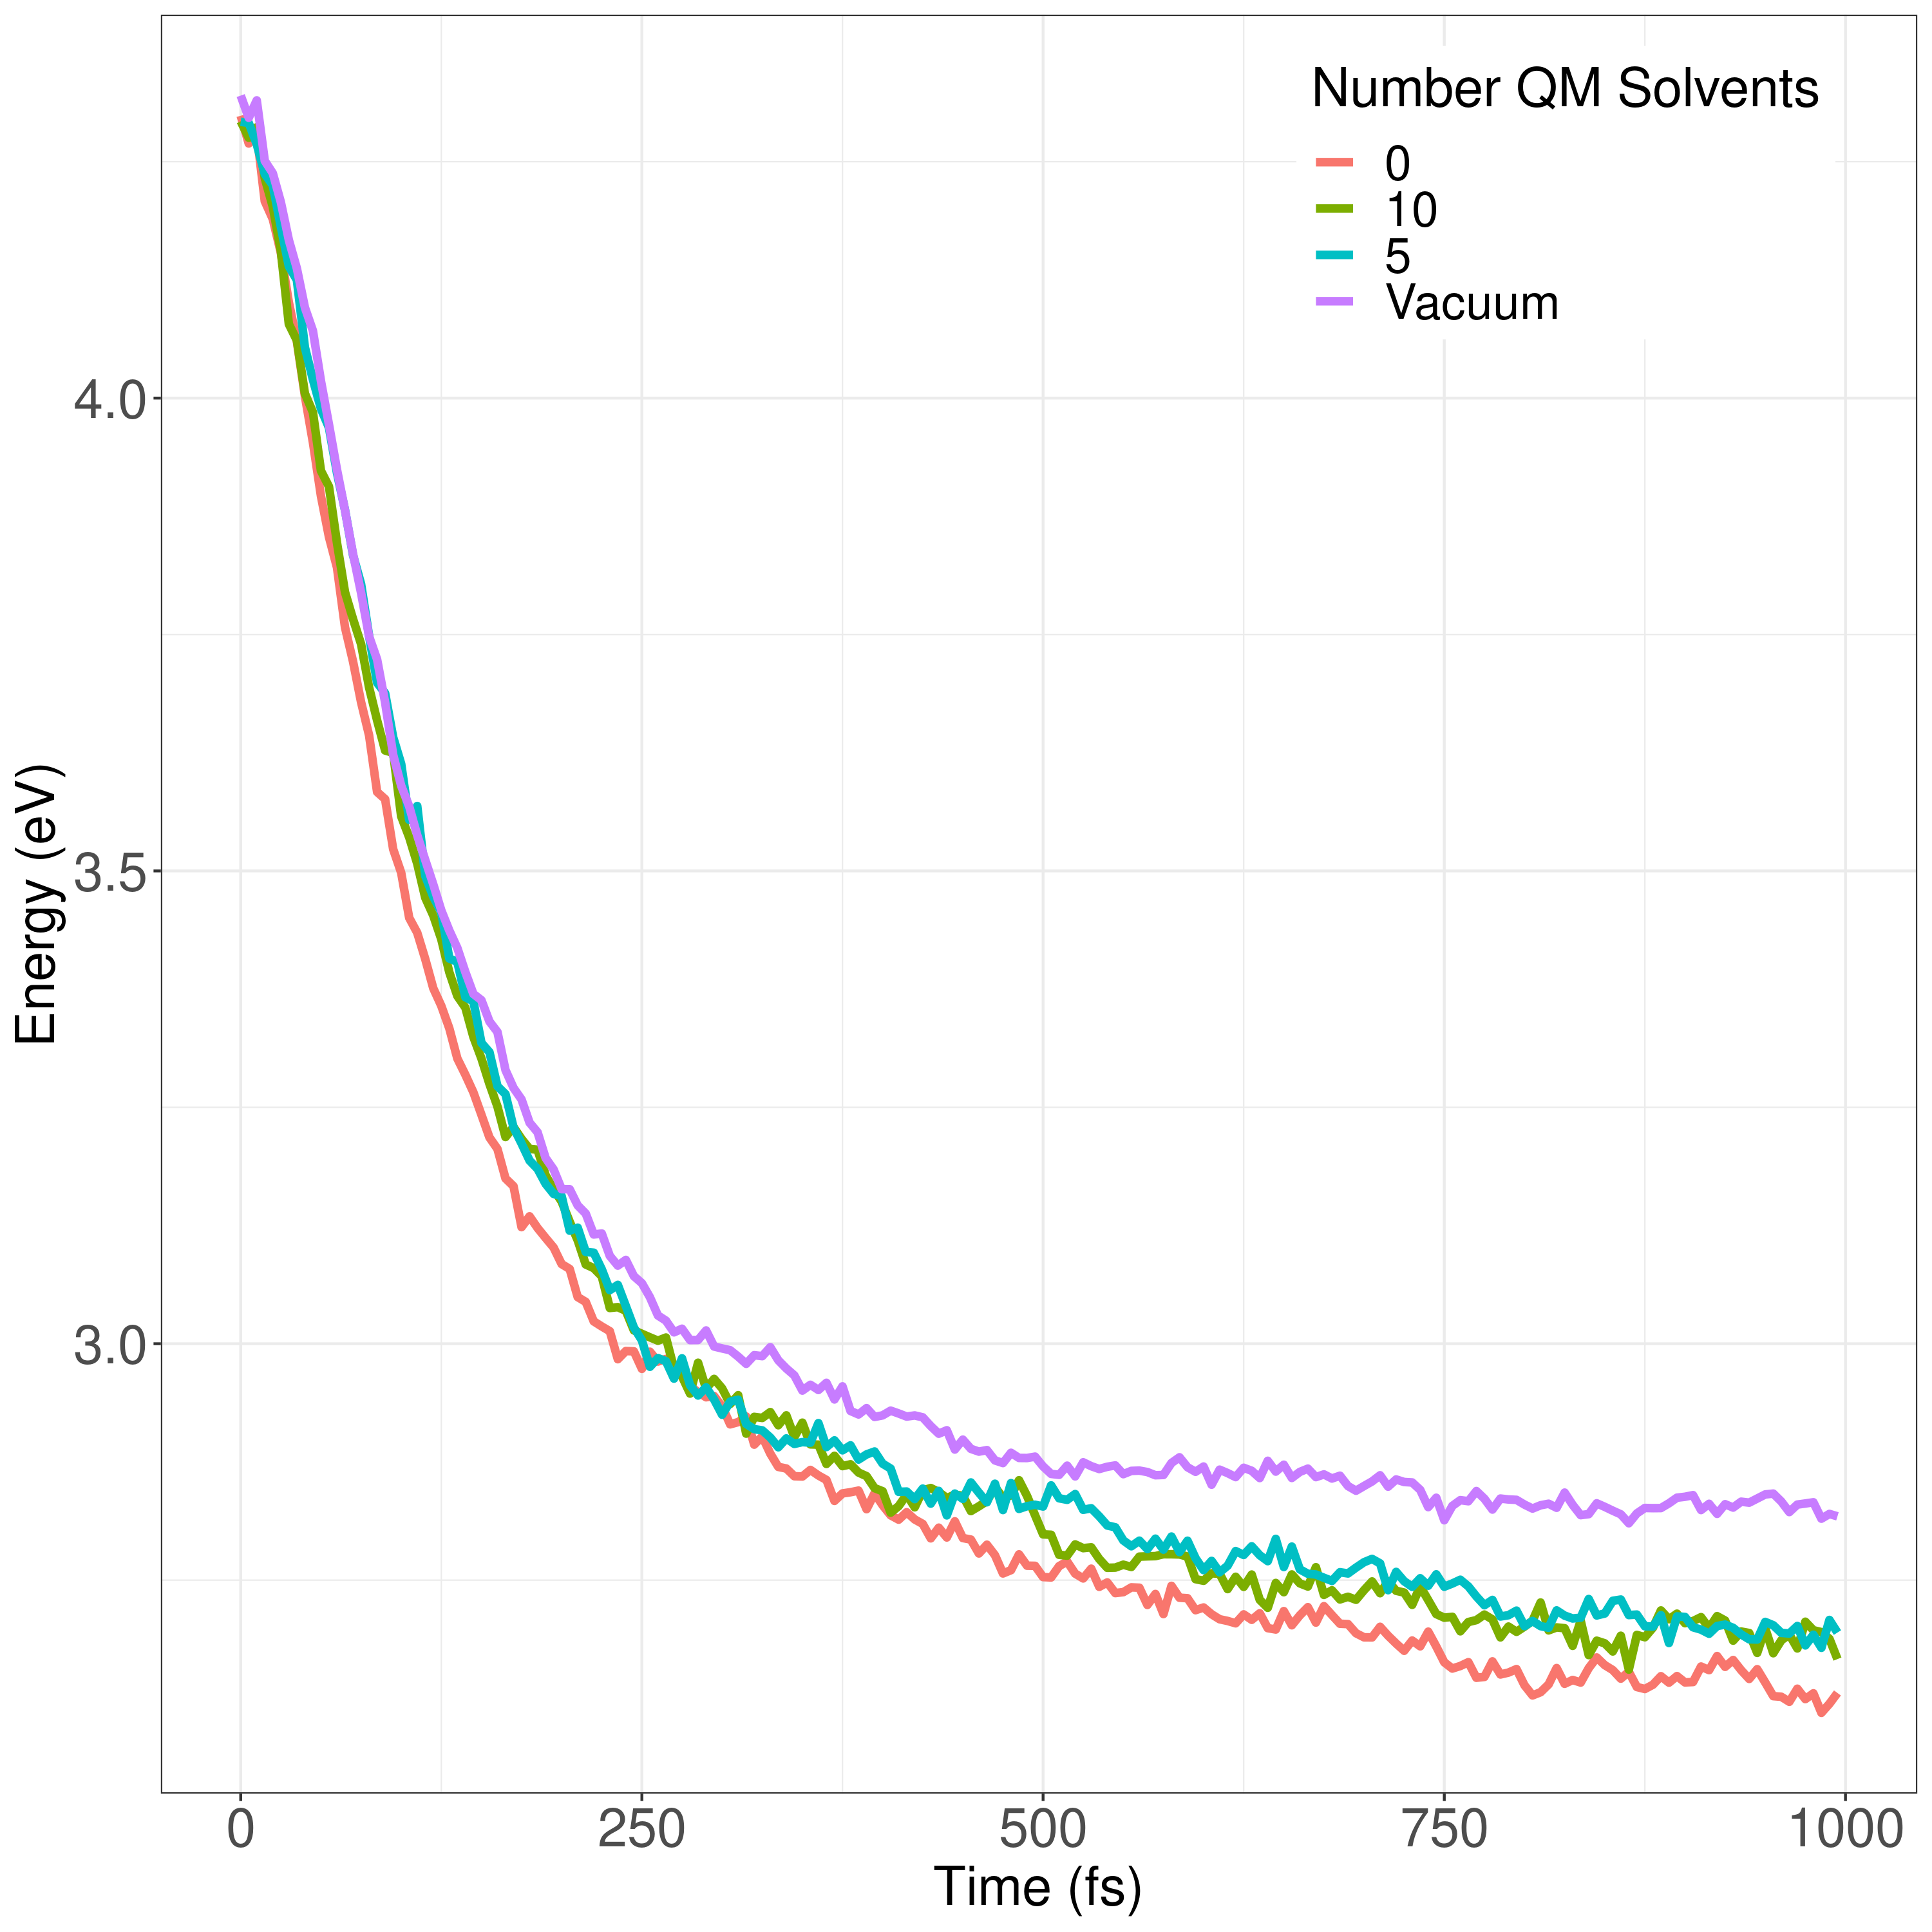
\includegraphics[width=0.5\textwidth]{../Paper2/Images/potential_energies/solvent_comparison.png}
  \captionof{figure}{Potential energy difference from the intial ground state during dynamics averaged over trajectories.}
  \label{}
\end{minipage}\bigskip

\subsection{Bond Length Alternation}

\subsection{Torsional Angle Relaxation}

\noindent
\begin{minipage}[c]{\textwidth}
  \centering
  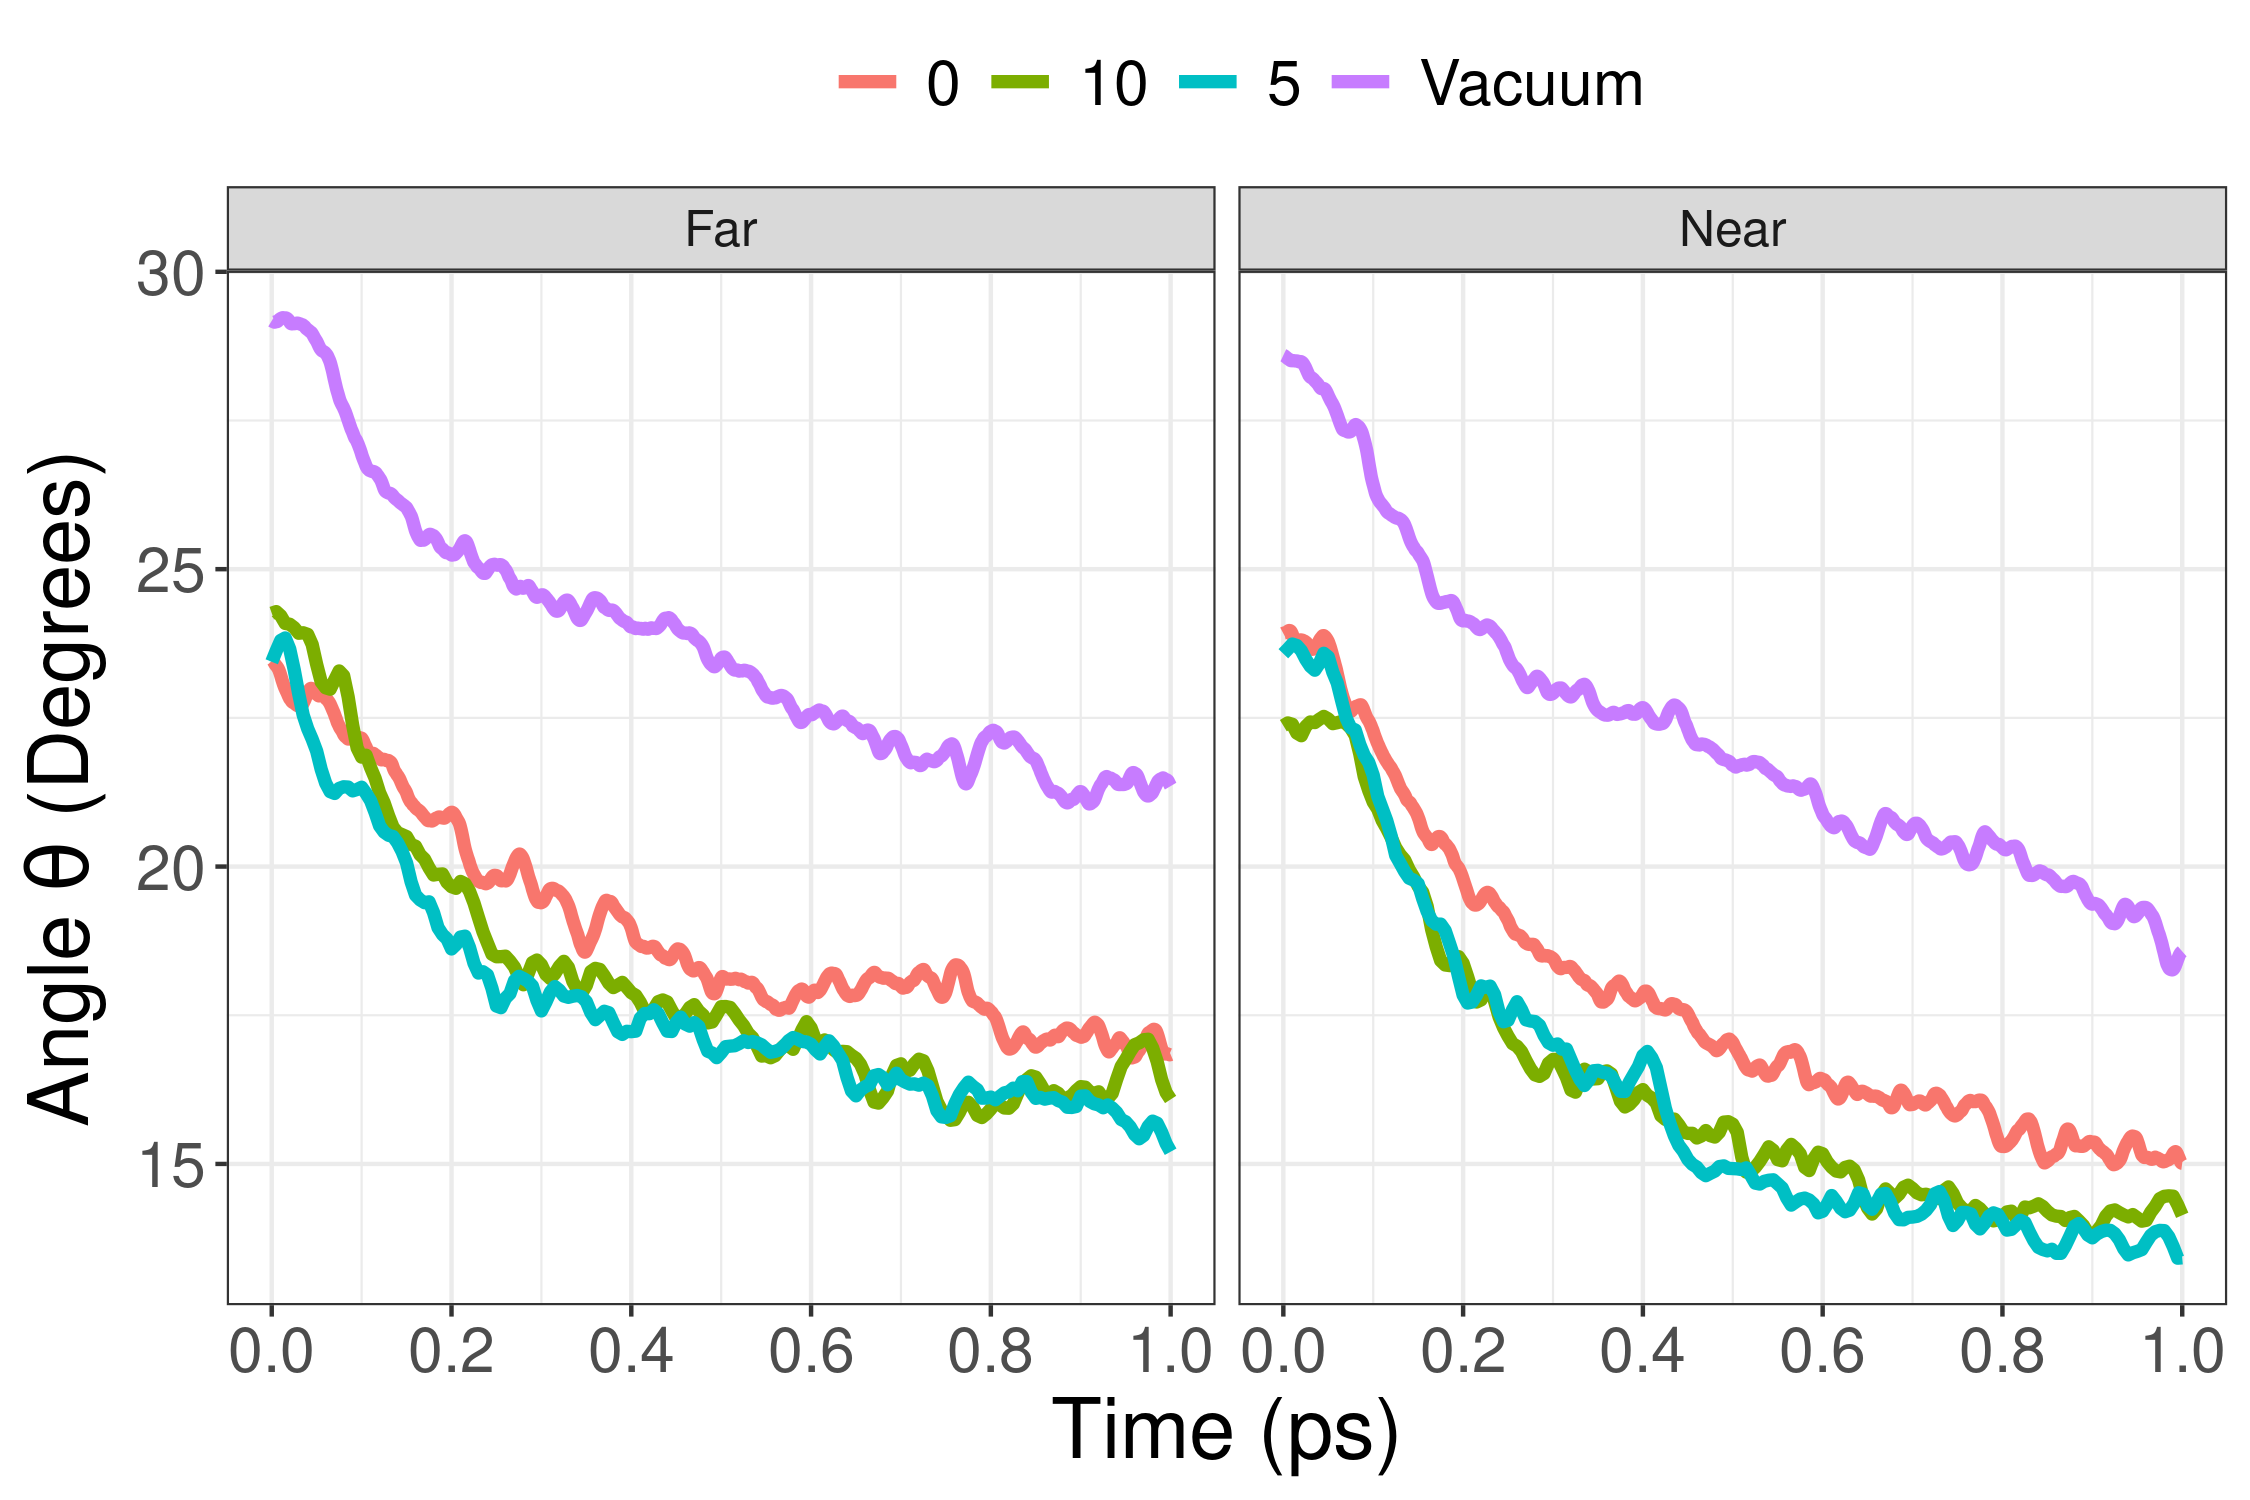
\includegraphics[width=5in]{../Paper2/Images/dihedral/solvent_comparison.png}
  \captionof{figure}{Dihedral angles of PPV\(_{3}\)-NO\(_{2}\) with varying number of solvents included in the QM region.}
  \label{dihedralNonadiabatic}
\end{minipage}\bigskip

\subsection{Widberg Bond Relaxation}

\subsection{Bond Orders}
\noindent
\begin{minipage}[c]{\textwidth}
  \centering
  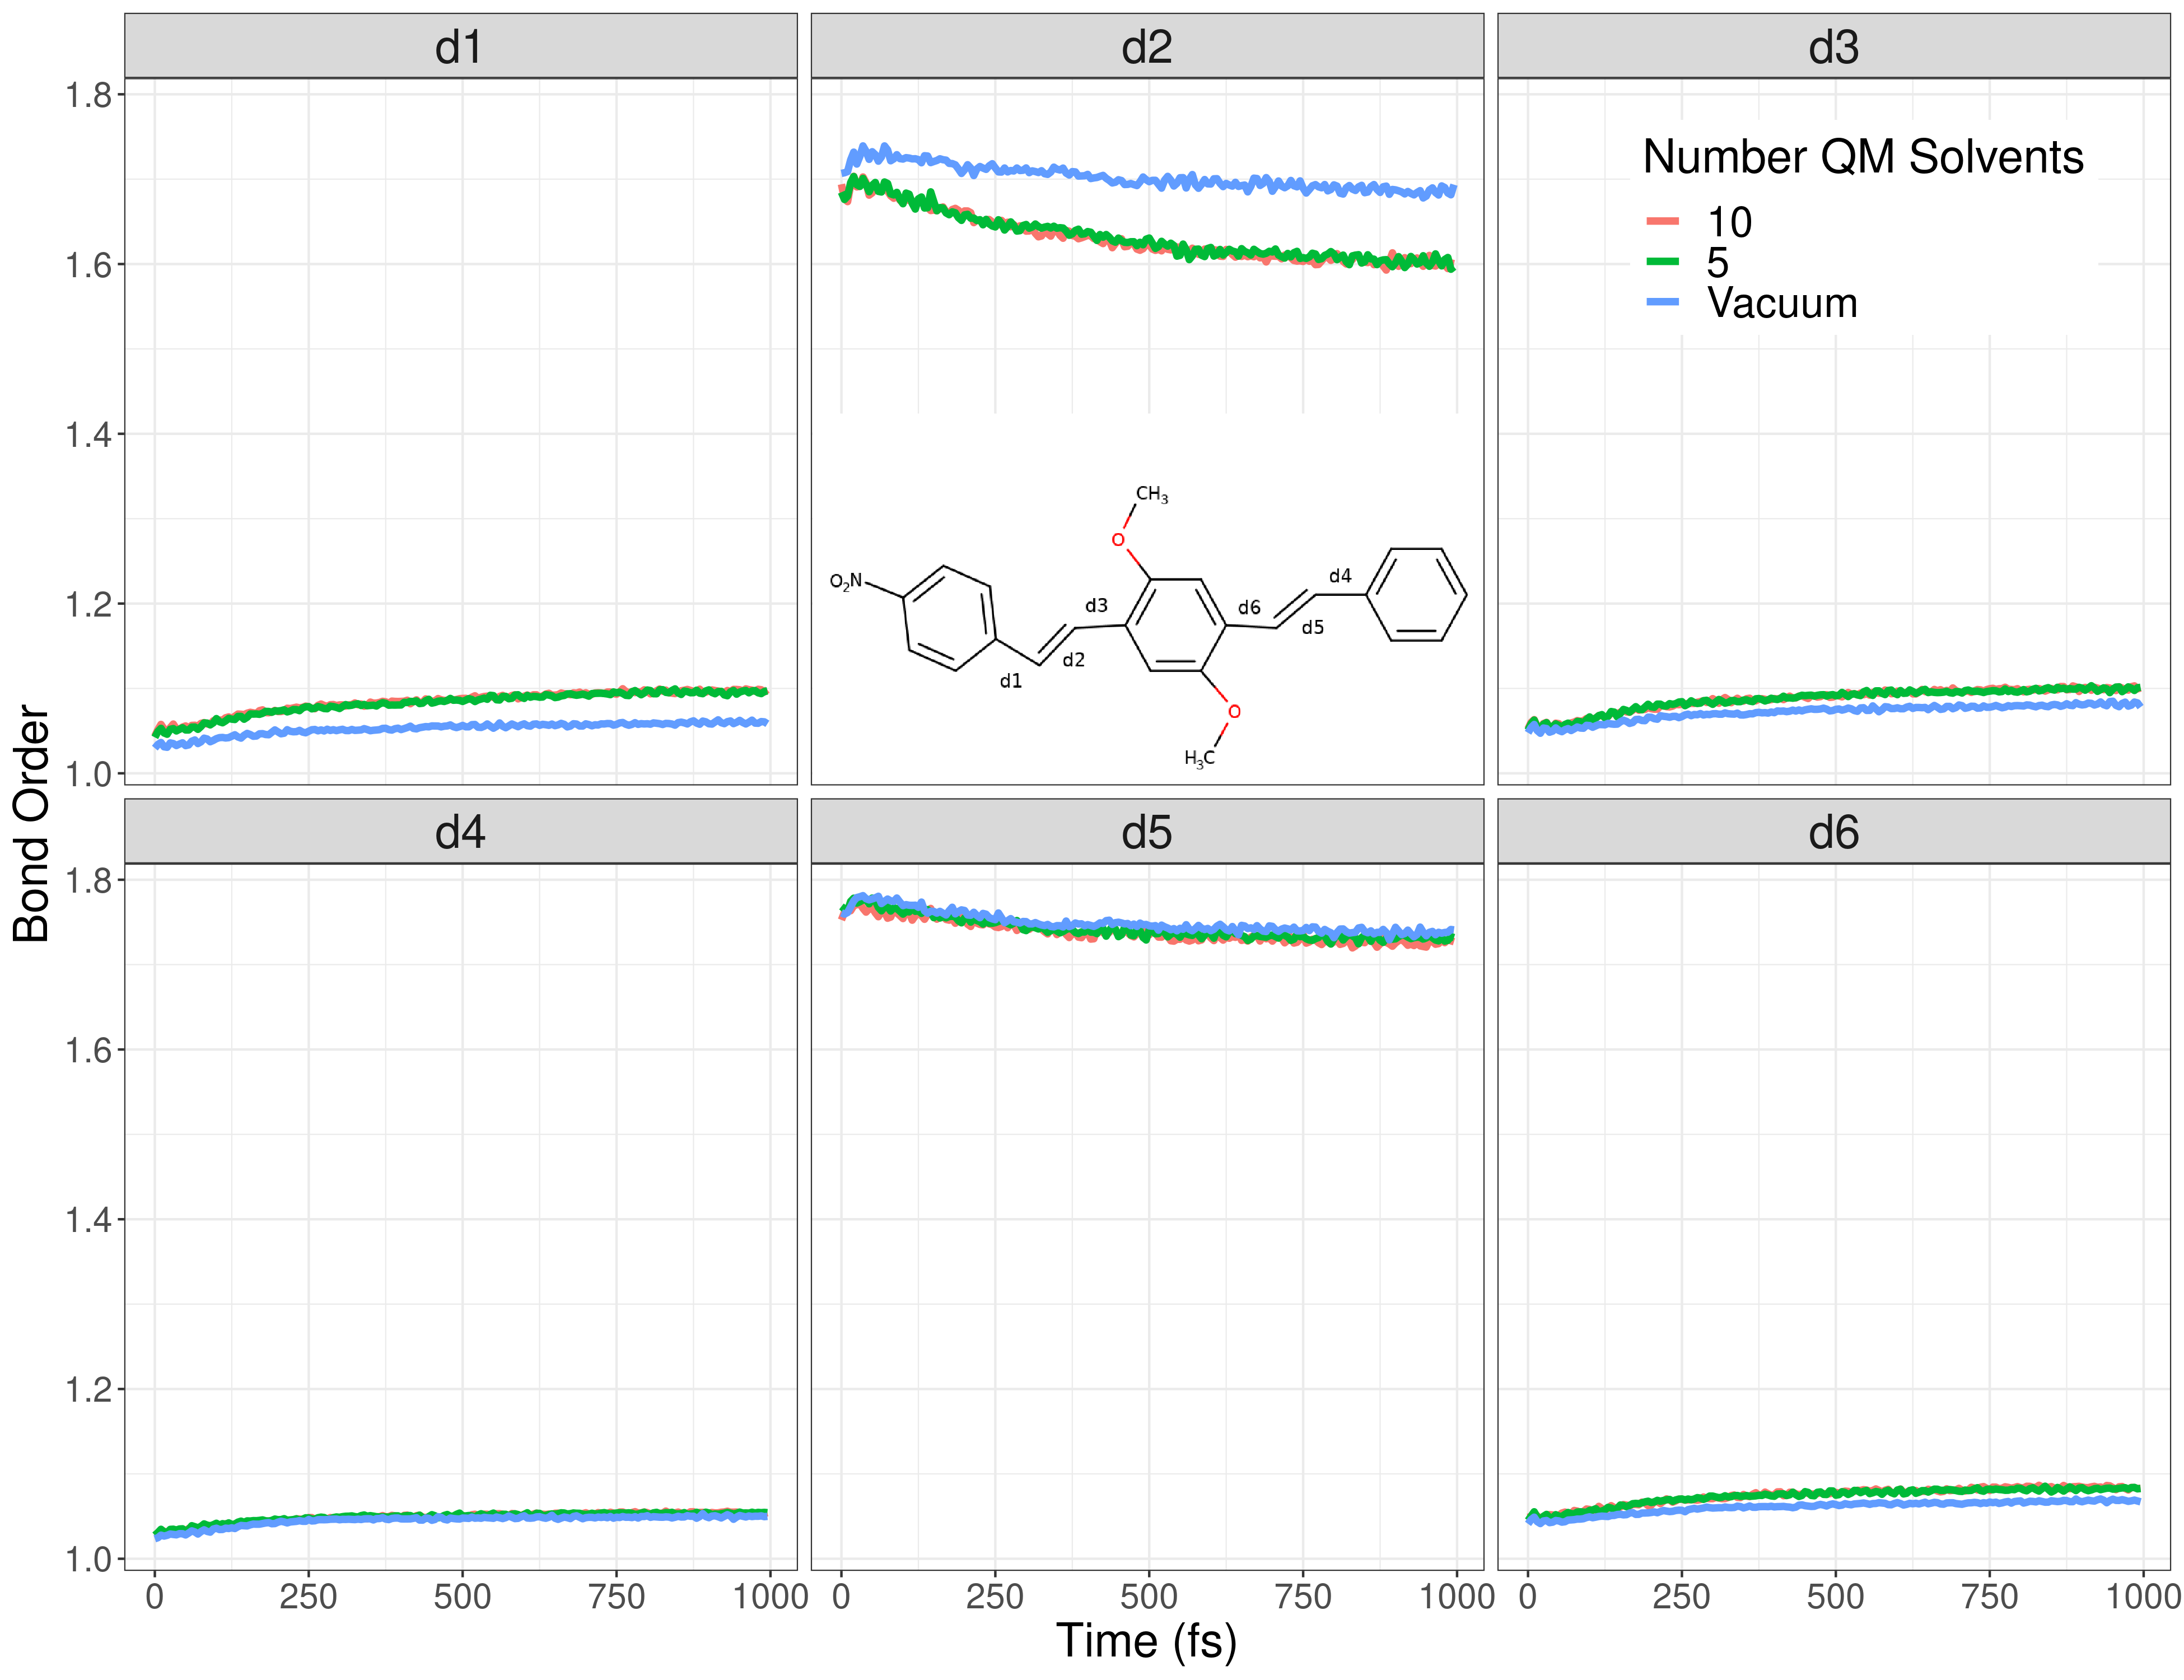
\includegraphics[width=5in]{../Paper2/Images/bond_order/solvent_comparison.png}
  \captionof{figure}[Wiberg Bond Orders in Nonadiabatic Dynamics]{The Wiberg Bond Orders averaged over the ensemble of trajectories for select bonds for PPV\(_3\)-NO\(_2\) with various number of solvents included in the QM region.}
  \label{bondOrderNonadiabatic}
\end{minipage}\bigskip
